% Flowchart of the spatial ignition probability methodology
\documentclass[border=2pt]{standalone}
\usepackage[scaled]{helvet}    
\renewcommand{\familydefault}{\sfdefault}
\usepackage[T1]{fontenc}
\usepackage[utf8]{inputenc}
\usepackage{tikz}
\usetikzlibrary{positioning,arrows.meta,fit,backgrounds,calc,shapes.geometric}

\begin{document}
\hyphenpenalty=10000\exhyphenpenalty=10000
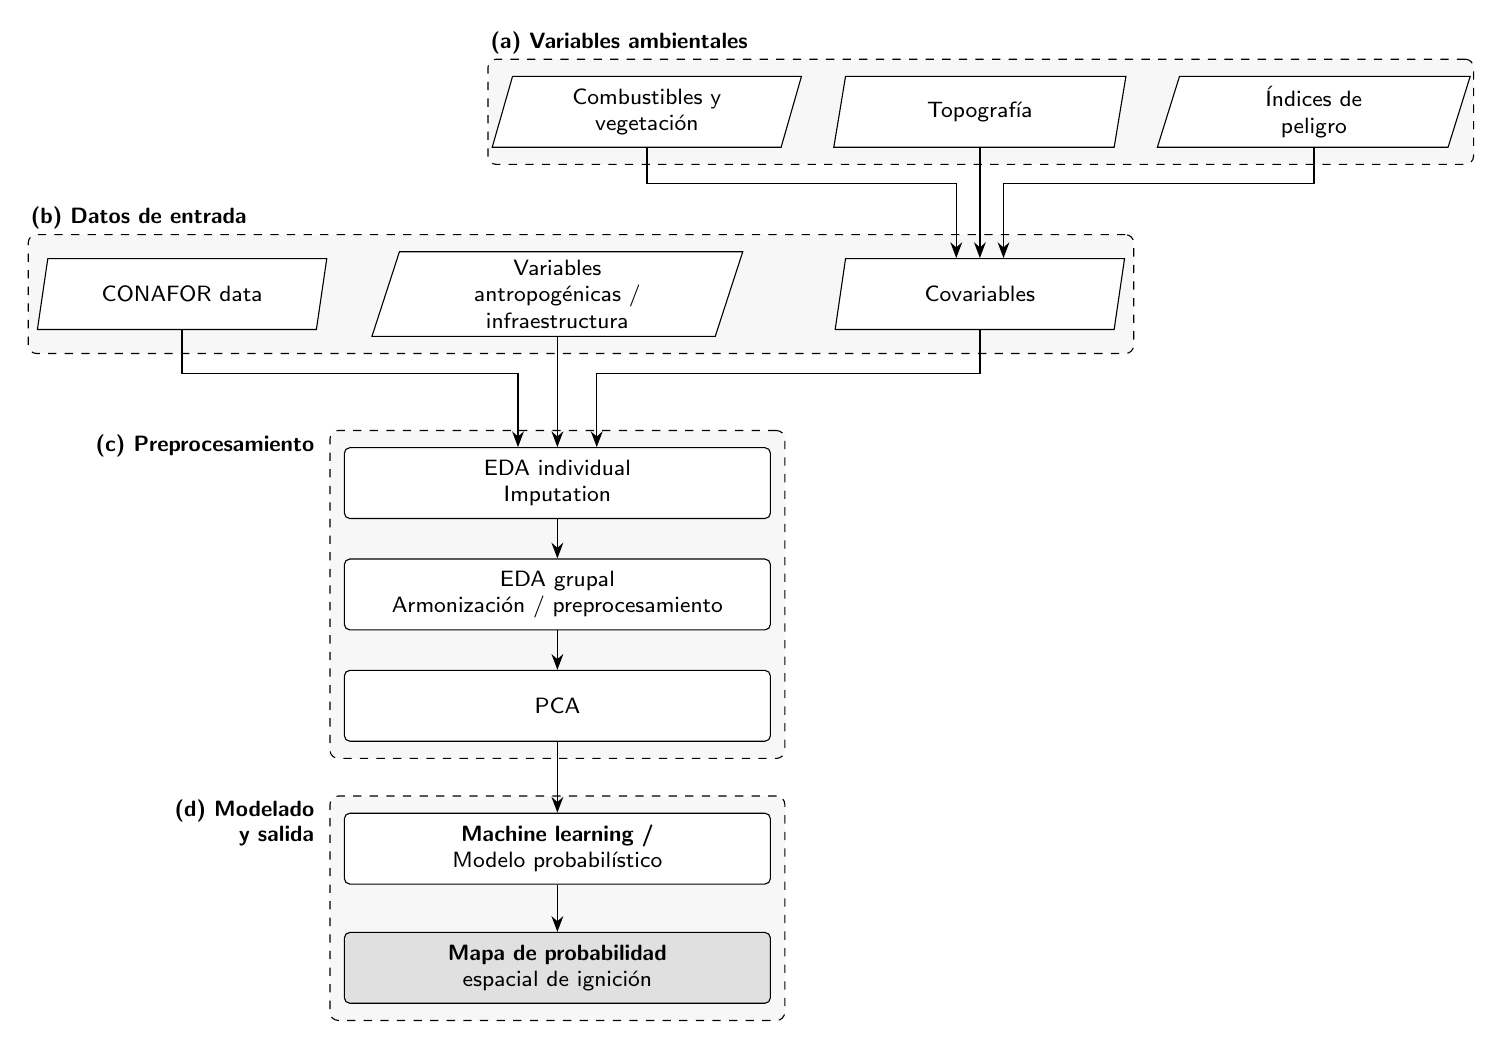
\begin{tikzpicture}[
  font=\fontsize{8}{9.5}\selectfont,
  % Estilo para entradas de datos (paralelogramos como en la imagen)
  io/.style={draw, trapezium, trapezium left angle=72, trapezium right angle=108,
             trapezium stretches=true, line width=0.4pt, align=center,
             text width=#1, minimum height=9mm, inner sep=3pt, fill=white},
  io/.default=34mm,
  % Estilo estándar de cajas de proceso de tu plantilla
  box/.style={draw, rounded corners=2pt, line width=0.4pt, align=center,
              text width=#1, minimum height=9mm, inner sep=3pt, fill=white},
  box/.default=46mm,
  % Estilo de salida final sombreada de tu plantilla
  out/.style={box=#1, fill=black!12},
  out/.default=46mm,
  arr/.style={-{Stealth[length=2mm]}, line width=0.5pt},
  stage/.style={draw, dashed, rounded corners=3pt, line width=0.4pt,
                inner sep=5pt, fill=black!3},
  lab/.style={font=\fontsize{8}{9}\selectfont\bfseries, anchor=south west, inner xsep=1pt, inner ysep=1.5pt}
]

%% ---------------- Etapa (a): Sub-fuentes de covariables ----------------
\node[io=32mm] (comb) {Combustibles y\\vegetación};
\node[io=32mm, right=6mm of comb] (topo) {Topografía};
\node[io=32mm, right=6mm of topo] (ind) {Índices de\\peligro};

%% ---------------- Etapa (b): Entradas principales ----------------
\node[io=32mm, below=14mm of topo] (cov) {Covariables};
\node[io=38mm, left=14mm of cov] (antrop) {Variables\\antropogénicas /\\infraestructura};
\node[io=32mm, left=8mm of antrop] (conafor) {CONAFOR data};

%% ---------------- Etapa (c): Preprocesamiento y reducción ----------------
\node[box=52mm, below=14mm of antrop] (eda_ind) {EDA individual\\Imputation};
\node[box=52mm, below=5mm of eda_ind] (eda_grp) {EDA grupal\\Armonización / preprocesamiento};
\node[box=52mm, below=5mm of eda_grp] (pca) {PCA};

%% ---------------- Etapa (d): Modelado y salida ----------------
\node[box=52mm, below=9mm of pca] (ml) {\textbf{Machine learning /}\\Modelo probabilístico};
\node[out=52mm, below=6mm of ml] (map) {\textbf{Mapa de probabilidad}\\espacial de ignición};

%% ---------------- Marcos de etapas (al fondo) ----------------
\begin{scope}[on background layer]
  \node[stage, fit=(comb)(topo)(ind), inner ysep=6pt] (s1) {};
  \node[stage, fit=(conafor)(antrop)(cov), inner ysep=6pt] (s2) {};
  \node[stage, fit=(eda_ind)(eda_grp)(pca), inner ysep=6pt] (s3) {};
  \node[stage, fit=(ml)(map), inner ysep=6pt] (s4) {};
\end{scope}

\node[lab] at (s1.north west) {(a) Variables ambientales};
\node[lab] at (s2.north west) {(b) Datos de entrada};
\node[lab, anchor=north east, align=right] at ($(s3.north west)+(-1.5mm,0)$) {(c) Preprocesamiento};
\node[lab, anchor=north east, align=right] at ($(s4.north west)+(-1.5mm,0)$) {(d) Modelado\\y salida};

%% ---------------- Flechas de conexión ----------------
% De sub-fuentes hacia Covariables
\draw[arr] (comb.south) -- ++(0,-4.5mm) -| ($(cov.north)+(-3mm,0)$);
\draw[arr] (topo.south) -- (cov.north);
\draw[arr] (ind.south) -- ++(0,-4.5mm) -| ($(cov.north)+(3mm,0)$);

% De entradas principales hacia EDA individual
\draw[arr] (conafor.south) -- ++(0,-5.5mm) -| ($(eda_ind.north)+(-5mm,0)$);
\draw[arr] (antrop.south) -- (eda_ind.north);
\draw[arr] (cov.south) -- ++(0,-5.5mm) -| ($(eda_ind.north)+(5mm,0)$);

% Flujo vertical central
\draw[arr] (eda_ind) -- (eda_grp);
\draw[arr] (eda_grp) -- (pca);
\draw[arr] (pca) -- (ml);
\draw[arr] (ml) -- (map);

\end{tikzpicture}
\end{document}
